\documentclass[12pt]{article}

\usepackage[L7x,T1]{fontenc}
\usepackage[lithuanian, english]{babel}
\usepackage[top = 2cm, bottom = 2cm, left = 3cm, right = 1.5cm, includefoot]{geometry}
\usepackage{mathptmx}
\usepackage{vwcol}  
\usepackage{sectsty}
\usepackage{setspace}
\usepackage{fancyhdr}
\usepackage{graphicx}


\pagestyle{fancy}
\fancyhead{}
\fancyfoot{}
\fancyfoot[R]{\thepage}
\renewcommand{\headrulewidth}{0pt}

\begin{document}
	\pagenumbering{gobble}
	\sectionfont{\fontsize{14}{15}\selectfont}
	\renewcommand{\baselinestretch}{1.5} 
	\renewcommand{\contentsname}{\hfil Turinys \hfil}
	\begin{center}
		VILNIAUS UNIVERSITETAS \\  
		MATEMATIKOS IR INFORMATIKOS FAKULTETAS \\ 
		PROGRAMŲ SISTEMŲ KATEDRA \\ 

		\vspace*{\fill}
			{\large \textbf{Prigramų sistemų inžinerijos darbas} \par} \bigskip
			\textbf{Software engineering work} \\ \bigskip
			Projektinis darbas 
		\vspace*{\fill}

		\begin{vwcol}[widths = {0.4, 0.4}, sep = 0cm, justify = raggedright, rule = 0pt]
			 Atliko:
			\newpage
			2 kurso 5 grupės studentai \\
			Toma Burneikaitė \\
			Žygimantas Stongvilas \\
			Mantas Jurčius \\
			Rimvydas Meškauskas \\ 
		\end{vwcol}
		\bigskip
		\begin{vwcol}[widths = {0.4, 0.4}, sep = 0cm, justify = raggedright, rule = 0pt]
			Darbo vadovas:
		\newpage
			asist., dr., Vytautas Valaitis
		\end{vwcol}
	\end{center}
	
	\begin{center}
		\mbox{}
		\vfill
		Vilnius - 2018
	\end{center}
	\newpage

	\pagenumbering{arabic}
	\setcounter{page}{2}

	\section*{\hfil Anotacija \hfil}
	
	Šiame projektiniame darbe pristatomas automobilių skelbimų programėlės AutoInf įgyvendinimas. \\
	Projektas AutoInf skirta  palengvinti automobilio paieškas internete. Programėlė, skirta mobiliesiems įrenginiams, suteikia galimybę vartotojui legviau rasti jį dominančią transporto priemonę, sujungdama visus skelbimus, esančius Europos automobilių pardavimo skelbimų puslapiuose. \\
	Programų sitemos architektūra apibrėžiama naudojantis 4+1 architektūros pjūvių modelį. Toliau pristatomi programos reikalavimai, bei pateikiama dalykinės srities analizė. 
	\newpage

	\tableofcontents
	\newpage

	\section*{\hfil Įvadas \hfil}
	\newpage

	\section*{\hfil Projektavimas \hfil}
		\subsection*{\hfil Užduotys ir jų vykdymo scenarijai \hfil}
			%\begin{figure}
				\includegraphics[width=\textwidth]{UserCase_AutoInf2.pdf}
			%	\caption{User Case diagrama}
			%\end{figure}

		\subsection*{\hfil Struktūrinis programų sistemos modelis \hfil}
			%\begin{figure}
			\subsubsection*{\hfil Klasių diagrama \hfil}
				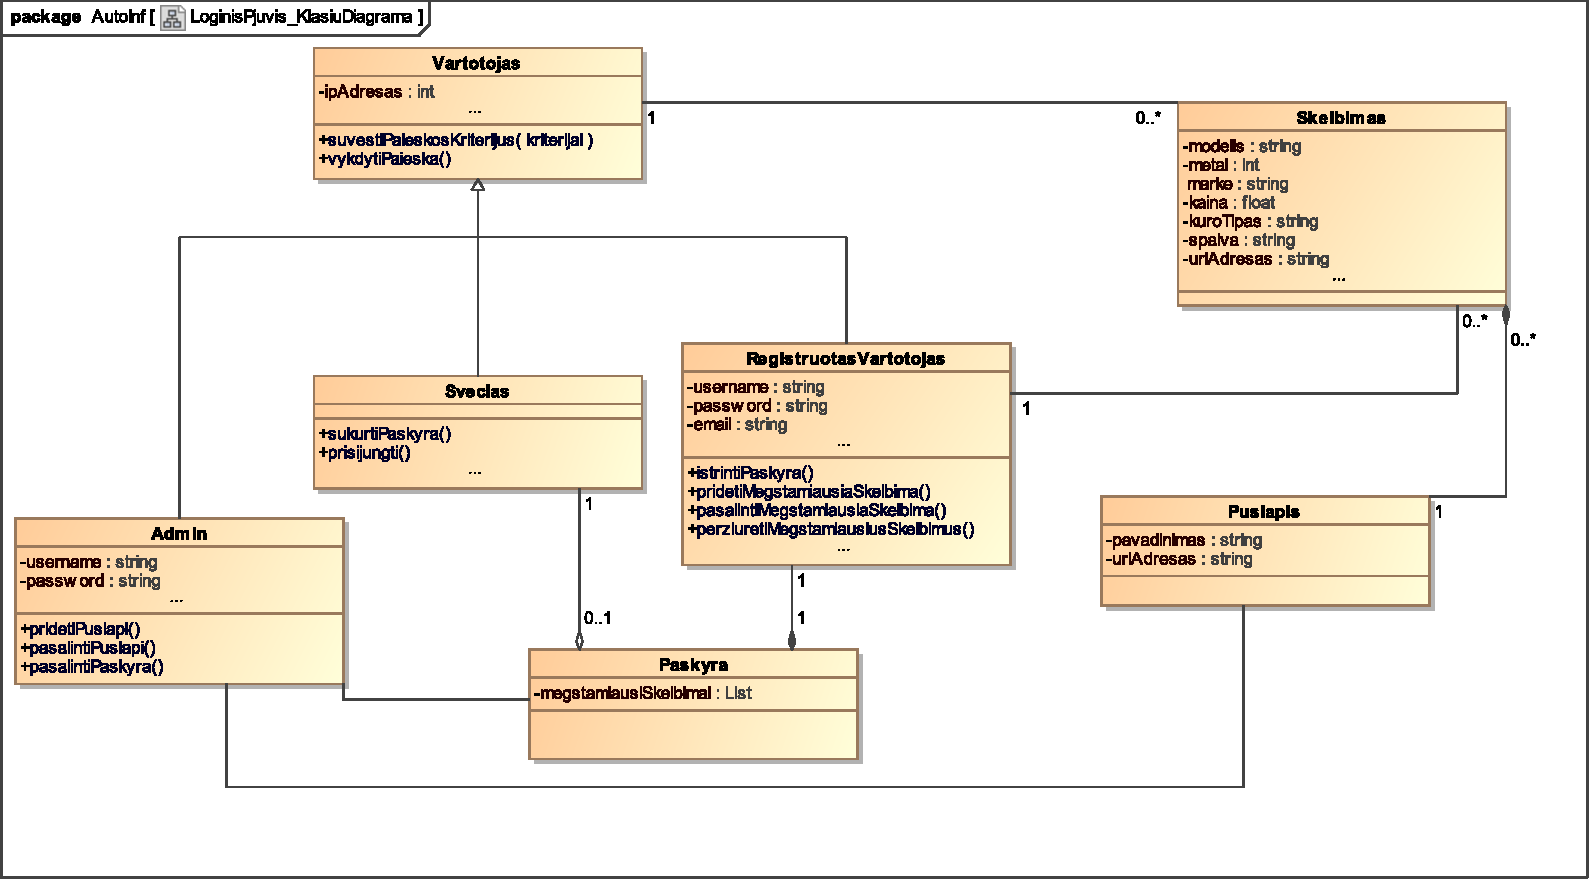
\includegraphics[width = \textwidth, angle = 0]{LoginisPjuvis_KlasiuDiagrama2.pdf}
			%	\caption{Klasiu diagrama}
			%\end{figure}

			\subsubsection*{\hfil Objektų diagrama \hfil}
				


\end{document}